\documentclass[11pt,a4paper]{article}

\usepackage[margin=2.5cm]{geometry}
\usepackage[T1]{fontenc}
\usepackage{lmodern}
\usepackage{microtype}
\usepackage{booktabs}
\usepackage{longtable}
\usepackage{xcolor}
\usepackage{listings}
\usepackage{amsmath}
\usepackage{amssymb}
\usepackage{enumitem}
\usepackage{tikz}
\usetikzlibrary{arrows.meta,positioning}
\usepackage[hidelinks]{hyperref}

\definecolor{codebg}{RGB}{247,247,247}
\definecolor{codekey}{RGB}{20,80,160}
\definecolor{codestr}{RGB}{150,60,20}
\definecolor{warnbg}{RGB}{255,248,235}
\definecolor{warnrule}{RGB}{200,140,40}

\lstdefinestyle{json}{
  basicstyle=\ttfamily\footnotesize,
  backgroundcolor=\color{codebg},
  breaklines=true, columns=fullflexible, keepspaces=true,
  showstringspaces=false, frame=single, framerule=0pt, framesep=6pt,
  xleftmargin=6pt, stringstyle=\color{codestr},
  literate=*{:}{{{\color{codekey}:}}}{1}{\{}{{{\color{codekey}\{}}}{1}{\}}{{{\color{codekey}\}}}}{1},
}
\lstdefinestyle{plain}{
  basicstyle=\ttfamily\footnotesize, backgroundcolor=\color{codebg},
  breaklines=true, columns=fullflexible, keepspaces=true,
  showstringspaces=false, frame=single, framerule=0pt, framesep=6pt, xleftmargin=6pt,
}
\lstset{style=json}

\newcommand{\code}[1]{\texttt{\small #1}}
\newcommand{\file}[1]{\texttt{\small #1}}

% ---- GitHub links to files in the repository ---------------------------------
\newcommand{\ghbase}{https://github.com/ArashMassoudieh/OpenHydroQual/blob/master}
\newcommand{\ghtree}{https://github.com/ArashMassoudieh/OpenHydroQual/tree/master}
\newcommand{\exfile}[1]{\href{\ghbase/#1}{\file{#1}}}
\newcommand{\exdir}[1]{\href{\ghtree/#1}{\file{#1}}}

% ---- a boxed caveat ----------------------------------------------------------
\newenvironment{caution}
  {\par\medskip\noindent
\begin{tikzpicture}\node[draw=warnrule,fill=warnbg,line width=0.8pt,
   rounded corners=2pt,inner sep=8pt,text width=\dimexpr\textwidth-20pt\relax,align=left]\bgroup}
  {\egroup;\end{tikzpicture}\par\medskip}

\title{\textbf{Culvert Modelling in OpenHydroQual}\\[0.3em]
       \large HDS-5 inlet control, outlet control, and storage-routed barrels}
\author{}
\date{}

\begin{document}
\maketitle
\vspace{-2.5em}

\begin{abstract}
\noindent
A culvert is not a pipe with a friction law. Its discharge is set by whichever
of two independent mechanisms is more restrictive: the geometry of the entrance,
which can pass only so much flow for a given headwater regardless of what
happens downstream, or the energy budget along the barrel, which depends on
tailwater. This document sets out how both mechanisms are formulated for
OpenHydroQual, how the FHWA HDS-5 inlet-control equations are inverted so that
discharge can be obtained explicitly from head, how the barrel is represented
as a storage-routed element between two open channels, and what the resulting
components do and do not claim to reproduce.
\end{abstract}

\tableofcontents

\section{Scope and conventions}

The components documented here live in \exfile{resources/culvert.json} and are
registered as the \emph{Culverts} template in
\exfile{resources/default\_templates.list}. Worked models are in
\exdir{Examples/Culvert}.

\subsection{Units}

OpenHydroQual solves internally in metres and days. Every discharge expression
in the templates therefore carries a factor of $86400$ converting
$\mathrm{m^3\,s^{-1}}$ to $\mathrm{m^3\,day^{-1}}$, and every occurrence of
$2g$ appears as the numeric constant $19.62\ \mathrm{m\,s^{-2}}$. Elevations,
inverts and heads share a single vertical datum with the connected channel
blocks.

\subsection{What the expression language permits}\label{sec:lang}

The formulation below is shaped by a hard constraint: quantities are declared as
algebraic expressions evaluated by \exfile{aquifolium/src/ExpressionNode.cpp},
and that evaluator offers no conditionals, no loops, and no implicit solves.
Everything must be written as a single explicit algebraic expression in terms of
other quantities. The available operations that matter here are

\begin{itemize}[nosep,leftmargin=1.4em]
  \item \code{\_min}, \code{\_max} --- binary only, so a three-way selection must be nested;
  \item \code{\_pos}$(x)=\max(x,0)$ and \code{\_hsd}$(x)=H(x)$, a hard step;
  \item \code{\_sqr}$(x)=\sqrt{\max(x,0)}$, a magnitude-only square root;
  \item \code{\_sqt}$(x)=\operatorname{sgn}(x)\sqrt{x^{2}/(|x|+10^{-4})}$, a
        \emph{signed, regularised} square root;
  \item \code{\_mon}$(a,b)=a/(a+b)$, a smooth saturating switch;
  \item the power operator, evaluated as $\mathrm{pow}(|a|,b)$, so the exponent
        may itself be an expression.
\end{itemize}

\noindent
\code{\_sqt} is the workhorse. A culvert must pass flow in either direction and
must remain differentiable as the driving head crosses zero, and
$\operatorname{sgn}(\Delta H)\sqrt{|\Delta H|}$ is not differentiable there. The
regularised form behaves as $\sqrt{\Delta H}$ away from the origin and as a
smooth ramp through it.

\section{Barrel geometry}

\subsection{Circular section}

For a circular barrel of diameter $D$ flowing at depth $d$, write $x=d/D$. The
templates use the polynomial fits already established elsewhere in the
OpenHydroQual component library (they appear in \code{Sewer\_pipe}), so that a
culvert and a sewer conduit describe the same section the same way:

\begin{align}
A(x) &= D^{2}\left(-0.910331972\,x^{3}+1.376045712\,x^{2}+0.319684423\,x\right),
\label{eq:circA}\\
P(x) &= D\left(5.486583\,x^{3}-8.60202\,x^{2}+6.1081605\,x\right).
\label{eq:circP}
\end{align}

\noindent
Equation~\eqref{eq:circA} is accurate: at $x=1$ it returns $0.785398\,D^{2}$,
which is $\pi D^{2}/4$ to six figures. Equation~\eqref{eq:circP} is not: at
$x=1$ it returns $2.9925\,D$ against the exact $\pi D=3.14159\,D$, an
underestimate of $4.8\%$. This propagates into the hydraulic radius and hence
into the friction term of outlet control; see
Section~\ref{sec:limitations}.

\subsection{Recovering depth from storage}\label{sec:invert}

The storage-routed barrel of Section~\ref{sec:barrel} carries volume as its
state and must recover depth from it. This inverts~\eqref{eq:circA}, which is
cubic in $x$ and has no convenient closed-form inverse. Writing
$u=A/A_{\mathrm{full}}$ for the fraction of the section that is wetted, the
templates use a quintic fit constrained to pass through both endpoints exactly:

\begin{equation}
\frac{d}{D}=1.9470734\,u-4.948471\,u^{2}+10.344915\,u^{3}
           -10.5243768\,u^{4}+4.1808594\,u^{5}.
\label{eq:circinv}
\end{equation}

\noindent
This is monotone on $u\in[0,1]$, exact at $u=0$ and $u=1$, and its worst error
against a numerical inversion of~\eqref{eq:circA} is $0.005\,D$, half a percent
of the diameter.

\subsection{Box section}

For a rectangular barrel of span $B$ and rise $H$ the area is exact,
$A=Bd$, and the depth inverts trivially. The wetted perimeter must grow from
$B$ at $d=0$ to $2(B+H)$ when the barrel runs full, while not counting the
soffit before the water reaches it. The templates use

\begin{equation}
P = B\left(1+\left(\frac{d}{H}\right)^{4}\right)+2d,
\label{eq:boxP}
\end{equation}

\noindent
which is exact at both ends and engages the soffit only as the barrel
approaches full: at half depth it gives $1.0625B+H$ against the free-surface
value $B+H$.

\section{Inlet control}\label{sec:inlet}

\subsection{The HDS-5 equations}

FHWA HDS-5 expresses inlet control as a relation between headwater and
discharge through the dimensionless discharge parameter

\begin{equation}
q^{*}=\frac{K_u\,Q}{A\,D^{0.5}},\qquad K_u=1.811\ \text{(SI)},
\label{eq:qstar}
\end{equation}

\noindent
in which $A$ is the \emph{full} barrel area and $D$ the barrel rise. There are
three forms. Unsubmerged Form (1) adds the specific head at critical depth
$H_c$; unsubmerged Form (2) omits it; the submerged form is a quadratic:

\begin{align}
\text{Form (1):}\quad & \frac{HW_i}{D}=\frac{H_c}{D}+K\,(q^{*})^{M}+K_sS,
\label{eq:form1}\\
\text{Form (2):}\quad & \frac{HW_i}{D}=K\,(q^{*})^{M},
\label{eq:form2}\\
\text{submerged:}\quad & \frac{HW_i}{D}=c\,(q^{*})^{2}+Y+K_sS.
\label{eq:sub}
\end{align}

\noindent
$S$ is the barrel slope and $K,M,c,Y$ are tabulated in HDS-5 Table~A.1
(reproduced in Section~\ref{sec:tablea1}) by barrel shape, material and inlet
edge treatment. The slope correction is $K_s=-0.5$ for all inlets except mitered
ones, which take $K_s=+0.7$. Note that Form~(2) carries \emph{no} slope term.

Rearranging Form~(1) to isolate the two discharge-dependent terms gives
$H_c/D+K(q^{*})^{M}=HW_i/D-K_sS$, so the templates work with
$\tau=HW_i/D+\lambda S$ where $\lambda=-K_s$. The parameter
\code{slope\_correction\_coeff} is therefore entered as $0.5$ in the normal case
and $-0.7$ for a mitered inlet.

The transition limits quoted by HDS-5 --- unsubmerged up to $Q/AD^{0.5}=3.5$
(1.93 SI), submerged above $4.0$ (2.21 SI) --- are two statements of the same
threshold on the dimensionless group $q^{*}$, since $1.811\times1.93=3.50$ and
$1.811\times2.21=4.00$. Comparing $q^{*}$ against $3.5$ and $4.0$ is thus
unit-independent and is what the templates do.

\subsection{Inverting for discharge}

HDS-5 is written to answer ``what headwater does this discharge require?''.
OpenHydroQual needs the opposite: the solver knows heads and must produce a
flow. Two of the three forms invert directly. From~\eqref{eq:sub},

\begin{equation}
q^{*}_{\mathrm{sub}}=\sqrt{\frac{HW/D-Y+0.5S}{c}},
\label{eq:invsub}
\end{equation}

\noindent
and from~\eqref{eq:form2},
$q^{*}_{(2)}=\left(\dfrac{HW/D}{K}\right)^{1/M}$. Both are single expressions.
Form (1) is the difficult one, because $H_c$ is the specific head at critical
depth \emph{for the discharge being sought}, making~\eqref{eq:form1} implicit.

\subsection{The critical-flow function}

Resolving Form (1) needs the map from a critical specific head to the discharge
that produces it. For a circular section at critical depth $d_c$, with
$\theta=2\arccos(1-2d_c/D)$, top width $T$ and area $A_c$,

\begin{equation}
Q_c=\sqrt{\frac{g A_c^{3}}{T}},\qquad
\frac{H_c}{D}=\frac{d_c}{D}+\frac{A_c}{2TD},
\label{eq:crit}
\end{equation}

\noindent
which is a parametric curve in $d_c$. Eliminating $d_c$ numerically and writing
$\chi=H_c/D$, the templates use

\begin{multline}
\frac{Q_c}{D^{5/2}}=\chi^{2}\bigl(1.9179351-0.4294827\,\chi-0.0636513\,\chi^{2}\\
   {}+0.0260040\,\chi^{3}-0.0431370\,\chi^{4}+0.0178421\,\chi^{5}\bigr),
\label{eq:critfit}
\end{multline}

\noindent
valid for $10^{-4}\le\chi\le1.6$ with a maximum \emph{relative} error of
$0.007\%$. The $\chi^{2}$ prefactor is not cosmetic: it carries the correct
small-depth asymptote, and normalising instead by $\chi^{3/2}$ degrades the fit
by three orders of magnitude. The diameter cancels, so~\eqref{eq:critfit} is a
pure function of $\chi$ and
$q^{*}_{\mathrm{crit}}(\chi)=K_u\,(Q_c/D^{5/2})/(\pi/4)$.

For a box section the same construction is exact and the geometry cancels
entirely. Critical flow gives $H_c=\tfrac32 d_c$ and $Q_c=B\sqrt{g\,d_c^{3}}$,
whence

\begin{equation}
q^{*}_{\mathrm{crit}}(\chi)=K_u\sqrt{g}\,
  \left[\min\!\left(\tfrac23\chi,\,1\right)\right]^{3/2}.
\label{eq:critbox}
\end{equation}

\subsection{Resolving Form (1)}

With $q^{*}_{\mathrm{crit}}$ available, write
$\tau=HW/D+\lambda S$ for the slope-corrected headwater ratio. Form
(1) states $H_c/D=\tau-K(q^{*})^{M}$, so the fixed point sought is

\begin{equation}
q^{*}=q^{*}_{\mathrm{crit}}\!\left(\tau-K\,(q^{*})^{M}\right).
\label{eq:fixedpoint}
\end{equation}

\noindent
Because $K(q^{*})^{M}$ is a small correction to $\tau$ over the unsubmerged
range, this converges --- but the undamped map is expansive at large $q^{*}$
and oscillates. The templates therefore unroll four \emph{damped} iterations,

\begin{equation}
q^{*}_{1}=q^{*}_{\mathrm{crit}}(\tau),\qquad
q^{*}_{k+1}=\min\!\left(\tfrac12\left[q^{*}_{k}
  +q^{*}_{\mathrm{crit}}\!\left(\tau-K(q^{*}_{k})^{M}\right)\right],\;q^{*}_{1}\right),
\label{eq:damped}
\end{equation}

\noindent
and take $q^{*}_{4}$. The clamp to $q^{*}_{1}$ is a rigorous bound, not a
safety hack: $K(q^{*})^{M}\ge0$ forces $H_c/D\le\tau$, and
$q^{*}_{\mathrm{crit}}$ is monotone, so the true root can never exceed the first
iterate. The argument of $q^{*}_{\mathrm{crit}}$ is additionally clamped to the
fitted range of~\eqref{eq:critfit}.

\subsection{The unsubmerged--submerged transition}

HDS-5 applies the unsubmerged form below $q^{*}=3.5$, the submerged form above
$q^{*}=4.0$, and interpolates between. The templates implement exactly that,

\begin{equation}
w=\min\!\left(\max\!\left(\frac{q^{*}_{\mathrm{sub}}-3.5}{0.5},\,0\right),\,1\right),
\qquad
q^{*}=(1-w)\,q^{*}_{\mathrm{unsub}}+w\,q^{*}_{\mathrm{sub}}.
\label{eq:blend}
\end{equation}

\begin{caution}
\textbf{The weight is keyed to $q^{*}_{\mathrm{sub}}$, not to
$q^{*}_{\mathrm{unsub}}$.} This matters. The submerged branch~\eqref{eq:invsub}
is closed-form and monotone everywhere, whereas the iterated unsubmerged branch
is only trustworthy inside its own regime. Keying the blend to the stable branch
means the unsubmerged value contributes \emph{exactly zero} above $q^{*}=4$,
where it is no longer meaningful. Keying it the other way --- the obvious
choice --- lets a diverging iterate leak into the answer at high headwater.
\end{caution}

\noindent
Finally the discharge follows by inverting~\eqref{eq:qstar}:
$Q_{\mathrm{inlet}} = N\,q^{*}A D^{0.5}/K_u$ for $N$ barrels.

\section{Outlet control}\label{sec:outlet}

Outlet control is the energy budget from headwater to tailwater: an entrance
loss, friction along the barrel, and a velocity-head loss at the exit. With
$k_e$ and $k_x$ the entrance and exit loss coefficients, $n$ Manning's
coefficient, $L$ the barrel length and $R$ the hydraulic radius,

\begin{equation}
Q_{\mathrm{outlet}}
 = A\,\text{\code{\_sqt}}\!\left(
   \frac{2g\,\Delta H}{k_e+k_x+2gn^{2}L\,R^{-4/3}}\right),
\label{eq:outlet}
\end{equation}

\noindent
signed by $\Delta H$ through the regularised root. The driving head is measured
between effective water surfaces referenced to the local inverts,
$\Delta H=\max(h_s,z_{\mathrm{in}})-\max(h_e,z_{\mathrm{out}})$, so that a
tailwater below the outlet invert produces a free outfall rather than a
spurious suction.

\subsection{The \texorpdfstring{$(d_c+D)/2$}{(dc+D)/2} grade line rule}\label{sec:hgl}

Equation~\eqref{eq:outlet} as written references the tailwater to the outlet
invert, which is wrong when the barrel is running full but the tailwater is low.
HDS-5 Section~3.2.2 records that backwater calculations show the extended
full-flow hydraulic grade line pierces the outlet plane midway between critical
depth and the top of the barrel, and prescribes

\begin{equation}
h_o=\max\!\left(TW,\ z_{\mathrm{out}}+\tfrac{d_c+D}{2}\right),\qquad d_c\le D.
\label{eq:hgl}
\end{equation}

\noindent
This needs critical depth for the discharge being sought, so like Form~(1) it is
implicit --- but the feedback is negative (raising $h_o$ lowers $Q$, which lowers
$d_c$, which lowers $h_o$), so it contracts. Three unrolled corrections suffice.
For a circular barrel, writing $\psi=Q/(\sqrt{g}D^{5/2})$ per barrel,

\begin{multline}
\frac{d_c}{D}=\sqrt{\psi}\,\bigl(0.9641769+0.3201129\,\psi-0.835724\,\psi^{2}\\
  {}+1.4329776\,\psi^{3}-1.4308019\,\psi^{4}+0.4947965\,\psi^{5}\bigr),
\label{eq:dcfit}
\end{multline}

\noindent
monotone with a worst error of $0.010\,D$, concentrated near $d_c/D\to1$ where
the cap $d_c\le D$ takes over anyway. For a box the relation is exact,
$d_c=(q^{2}/g)^{1/3}$ with $q$ the discharge per unit span.

\subsection{Why the rule must be gated, and gated widely}\label{sec:gate}

HDS-5 is explicit that~\eqref{eq:hgl} is an approximation with a limited range:
it ``can only be used if the barrel flows full for most of its length'', ``should
not be used if the inlet is not submerged'', and gives adequate results only down
to a headwater of $0.75D$. Applying it unconditionally would impose a large
spurious backwater on a nearly empty barrel. The templates therefore ramp it in
with a weight

\begin{equation}
\gamma=\min\!\left(\max\!\left(\frac{(h_s-z_{\mathrm{out}})/D-\gamma_{\mathrm{lo}}}
  {\gamma_{\mathrm{hi}}-\gamma_{\mathrm{lo}}},0\right),1\right),
\qquad
h_o^{\mathrm{eff}}=TW+\gamma\,\text{\code{\_pos}}\!\left(h_o-TW\right).
\label{eq:gate}
\end{equation}

\begin{caution}
\textbf{The upper limit is $1.8$, not the $1.2$ HDS-5 implies, and the reason is
numerical.} Over the ramp the grade line rises by up to $(d_c+D)/2\approx0.85D$
while the barrel head rises by only $(\gamma_{\mathrm{hi}}-\gamma_{\mathrm{lo}})D$.
If the band is narrower than about $0.85$, the driving head \emph{falls} as the
barrel fills: the outlet rating curve turns non-monotonic and the storage balance
acquires up to three simultaneous steady states. Sweeping the band width confirms
the fold and the extra roots vanish together at a width of $1.05$. Both limits
are exposed as \code{hgl\_rule\_lower} and \code{hgl\_rule\_upper}; narrowing the
band towards HDS-5's nominal $1.2$ reintroduces the multiple roots.
\end{caution}

\section{Combining the two controls}

The governing discharge is the more restrictive of the two mechanisms. HDS-5
computes the headwater each requires at a given $Q$ and takes the larger; the
templates compute the capacity each permits at a given head and take the
smaller. These are equivalent whenever both rating curves are monotone, which
they are. Preserving the sign,

\begin{equation}
Q=\min\!\left(Q_{\mathrm{inlet}},\,|Q_{\mathrm{outlet}}|\right)
  \cdot\frac{Q_{\mathrm{outlet}}}{|Q_{\mathrm{outlet}}|+\varepsilon},
\qquad \varepsilon=10^{-6},
\label{eq:combine}
\end{equation}

\noindent
which is continuous through $Q_{\mathrm{outlet}}=0$ and avoids
$\operatorname{sgn}$, whose discontinuity would otherwise sit exactly where the
solver spends its time.

\section{The storage-routed barrel}\label{sec:barrel}

\subsection{Layout}

A culvert between two open channels is represented as three objects: an inlet
transition link carrying inlet control and the entrance loss, a barrel block
carrying volume, and an outlet transition link carrying barrel friction and the
exit loss.

\begin{center}
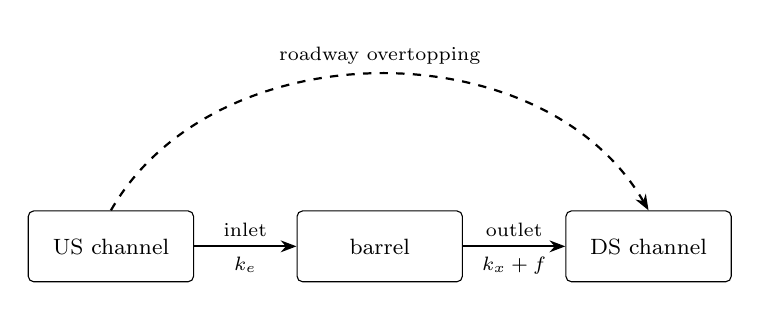
\begin{tikzpicture}[node distance=6mm and 13mm,
  blk/.style={draw,rounded corners=2pt,minimum height=9mm,minimum width=21mm,font=\footnotesize,align=center},
  lnk/.style={-{Stealth[length=2mm]},thick}]
  \node[blk] (us) {US channel};
  \node[blk,right=of us] (b) {barrel};
  \node[blk,right=of b] (ds) {DS channel};
  \draw[lnk] (us) -- node[above,font=\scriptsize]{inlet} node[below,font=\scriptsize]{$k_e$} (b);
  \draw[lnk] (b) -- node[above,font=\scriptsize]{outlet} node[below,font=\scriptsize]{$k_x+f$} (ds);
  \draw[lnk,dashed] (us.north) to[out=60,in=120] node[above,font=\scriptsize]{roadway overtopping} (ds.north);
\end{tikzpicture}
\end{center}

\noindent
Splitting the losses across two links is not an approximation. At steady state
the same $Q$ passes both, so
$\Delta H_1/k_e=\Delta H_2/(k_x+f)$ with $\Delta H_1+\Delta H_2=HW-TW$, giving
$\Delta H_1=k_e(HW-TW)/(k_e+k_x+f)$ and hence exactly~\eqref{eq:outlet}. The
split is verified numerically in Section~\ref{sec:verification}.

\begin{caution}
The entrance-loss term on the inlet link uses the \emph{full} barrel area, not
the barrel's current wetted area. Using the current area deadlocks the model: an
empty barrel has zero area, so the entrance-loss capacity is zero, so no water
can ever enter. In the partially-full regime inlet control governs anyway, and
in the full regime the full area is the correct one.
\end{caution}

\subsection{Surcharge and the Preissmann slot}

Once the barrel runs full it can carry pressure head above its crown, but a
free-surface storage element cannot represent that: storage saturates at
$A_{\mathrm{full}}L$ and stage stops responding. The templates use the standard
device of a narrow virtual slot above the crown of width $\sigma D$, so that

\begin{equation}
h = z_b + d(\mathcal{S}) + \frac{\max(\mathcal{S}-\mathcal{S}_{\mathrm{full}},0)}
     {N L \sigma D},
\label{eq:slot}
\end{equation}

\noindent
with $\sigma$ exposed as \code{slot\_width\_ratio}. A narrow slot is more
physically faithful and stiffer to solve; the default $\sigma=0.02$ trades
towards fidelity, and widening it is the first thing to try if a surcharging
model struggles to converge.

\section{Roadway overtopping and flow accounting}

When headwater exceeds the road crest the embankment acts as a broad-crested
weir. HDS-5 Equation~3.9 gives $Q_o=C_d L\,HW_r^{1.5}$ with $C_d=k_tC_r$, where
$C_r$ is the free-flow coefficient from Figure~3.11A/B and $k_t$ the correction
for downstream submergence from Figure~3.11C. HDS-5 also notes
$C_d(\mathrm{SI})=0.552\,C_d(\mathrm{English})$, so the deep-overtopping value
of about $3.1$ in US units becomes the default $C_r=1.7$ used here.

Because $k_t$ is published as a graph rather than an equation, it is exposed as
the input \code{road\_submergence\_factor} (default $1.0$, a free overfall)
rather than fitted, and the diagnostic \code{road\_submergence\_ratio} is
written to the output so that the tailwater encroachment can be checked against
Figure~3.11C. The two paths are computed separately and reported separately, so
that the split between them is auditable:

\begin{equation}
Q_{\mathrm{road}}=k_t C_r B_r\left(\text{\code{\_pos}}(h_s-z_r)^{3/2}
                              -\text{\code{\_pos}}(h_e-z_r)^{3/2}\right),
\label{eq:road}
\end{equation}

\noindent
signed, and continuous as either side crosses the crest. In the single-link
variants the quantities \code{culvert\_flow} (all barrels) and
\code{overtopping\_flow} are both written to the output, together with
\code{overtopping\_fraction}, and

\begin{equation}
\code{flow}=\code{culvert\_flow}+\code{overtopping\_flow}
\end{equation}

\noindent
is always the \emph{total} --- it is the quantity the storage balances
aggregate. In the routed layout the roadway is a separate
\code{Roadway\_Overtopping} link and is therefore reported on its own.

\section{Numerical considerations}

Three choices in the templates exist purely to keep the implicit solver
well-behaved, and are worth recording because they are not obvious from the
hydraulics.

\begin{enumerate}[leftmargin=1.5em]
\item \textbf{Smooth switches over hard ones.} Regime blending uses
      \code{\_mon} and clamped linear ramps rather than \code{\_hsd}. A
      Heaviside step has zero derivative everywhere and a jump at the
      threshold, which stalls a Newton iteration sitting on it.

\item \textbf{Upwinding without $\operatorname{sgn}$.} Where a quantity must be
      taken from the upstream side, the templates use the continuous weight
      $w=\tfrac12+\tfrac12\,\Delta H/(|\Delta H|+10^{-3})$, which tends to $1$
      and $0$ away from the origin and passes smoothly through it.

\item \textbf{Floors belong in denominators, never in flow terms.} An early
      version floored the outlet link's flow area at $10^{-4}\,\mathrm{m^2}$ to
      protect the velocity calculation. Because that area multiplies into the
      discharge, a drained barrel then leaked about
      $5\times10^{-6}\,\mathrm{m^3\,s^{-1}}$ indefinitely and storage drifted
      negative. The area entering \code{flow} is now unfloored --- it is
      legitimately zero when the barrel is dry --- and the floor appears only
      in the denominator of \code{velocity}.
\end{enumerate}

\section{Components}

\subsection{Types}

\begin{longtable}{@{}p{0.33\textwidth}p{0.08\textwidth}p{0.51\textwidth}@{}}
\toprule
\textbf{Type} & \textbf{Kind} & \textbf{Role}\\
\midrule
\endhead
\code{Culvert Barrel (Circular)} & block & Storage-routed circular barrel; carries volume, stage, section geometry and the friction coefficient.\\
\code{Culvert Barrel (Box)} & block & As above for a rectangular section.\\
\code{Channel\_to\_culvert (Circular)} & link & Inlet transition: HDS-5 inlet control plus entrance loss.\\
\code{Channel\_to\_culvert (Box)} & link & As above, using the exact box critical-flow relation.\\
\code{Culvert\_to\_channel (Circular)} & link & Outlet transition: barrel friction, exit loss and the $(d_c+D)/2$ rule.\\
\code{Culvert\_to\_channel (Box)} & link & As above, using the exact rectangular critical-depth relation.\\
\code{Roadway\_Overtopping} & link & Weir flow over the embankment, connecting the two channels directly.\\
\code{Circular Culvert} & link & Lumped single-link culvert: both controls in one connector, no barrel storage.\\
\code{Box Culvert} & link & As above for a rectangular section.\\
\bottomrule
\end{longtable}

\noindent
The two layouts are alternatives. The lumped link is appropriate for short
culverts where barrel storage is negligible; the routed barrel adds attenuation
and gives constituents a real residence time inside the structure. The outlet
link and the roadway link are shape-generic because the barrel blocks expose a
common vocabulary (\code{barrel\_rise}, \code{barrel\_area},
\code{inlet\_crest\_width}, \code{friction\_loss\_coeff}), so only the
inlet link needs a per-shape variant. The outlet link became shape-specific only
when the $(d_c+D)/2$ rule of Section~\ref{sec:hgl} was added, since critical
depth is a property of the section.

\subsection{Barrel parameters}

\begin{longtable}{@{}p{0.30\textwidth}p{0.42\textwidth}p{0.09\textwidth}p{0.09\textwidth}@{}}
\toprule
\textbf{Parameter} & \textbf{Meaning} & \textbf{Default} & \textbf{Unit}\\
\midrule
\endhead
\code{Number\_of\_barrels} & Number of barrels & 1 & -- \\
\code{diameter} & Barrel diameter (circular) & -- & m \\
\code{barrel\_width} & Span (box) & -- & m \\
\code{barrel\_height} & Rise (box) & -- & m \\
\code{length} & Barrel length & -- & m \\
\code{inlet\_invert} & Invert elevation at the upstream face & -- & m \\
\code{outlet\_invert} & Invert elevation at the downstream face & -- & m \\
\code{ManningCoeff} & Manning's roughness coefficient & 0.013 & -- \\
\code{inflow} & Optional direct inflow time series & -- & m$^3$/day \\
\code{inlet\_crest\_width\_factor} & Legacy crest-width factor (circular) & 0.65 & -- \\
\code{slot\_width\_ratio} & Preissmann slot width, as a fraction of the rise & 0.02 & -- \\
\code{depth} & Initial water depth & -- & m \\
\bottomrule
\end{longtable}

\subsection{Inlet link parameters}

\begin{longtable}{@{}p{0.30\textwidth}p{0.42\textwidth}p{0.09\textwidth}p{0.09\textwidth}@{}}
\toprule
\textbf{Parameter} & \textbf{Meaning} & \textbf{Default} & \textbf{Unit}\\
\midrule
\endhead
\code{entrance\_loss\_coeff} & HDS-5 $k_e$ & 0.5 & -- \\
\code{HDS5\_K} & Table A.1 coefficient $K$ & 0.0098 & -- \\
\code{HDS5\_M} & Table A.1 exponent $M$ & 2.0 & -- \\
\code{HDS5\_c} & Table A.1 coefficient $c$ & 0.0398 & -- \\
\code{HDS5\_Y} & Table A.1 coefficient $Y$ & 0.67 & -- \\
\code{HDS5\_form1\_switch} & $1$ for equation Form (1), $0$ for Form (2) & 1 & -- \\
\code{slope\_correction\_coeff} & $\lambda$ in $\tau=HW/D+\lambda S$; $0.5$ normally, $-0.7$ mitered & 0.5 & -- \\
\bottomrule
\end{longtable}

\begin{caution}
\textbf{The defaults are one row of Table~A.1 each; change them to match your
inlet.} The circular templates default to Chart~1 scale~1 (square edge with
headwall) and the box templates to Chart~8 scale~1 (30--75$^\circ$ wingwall
flares). Every other configuration has its own constants \emph{and possibly a
different equation form} --- note in Section~\ref{sec:tablea1} that all
circular entries are Form~(1) while box Charts~9--13 are Form~(2), which
requires \code{HDS5\_form1\_switch}${}=0$.
\end{caution}

\section{HDS-5 Table A.1 constants}\label{sec:tablea1}

Reproduced from HDS-5 Third Edition, Table~A.1 (\emph{Constants for Inlet
Control Equations for Charts in Appendix G}), for the circular and rectangular
shapes these components cover. Tapered-inlet and non-circular rows (Charts
55--59 and Tables A.2--A.6) are omitted, as are shapes the templates do not
represent.

\begin{longtable}{@{}llcp{0.30\textwidth}ccccc@{}}
\toprule
\textbf{Chart} & \textbf{Shape/Material} & \textbf{Sc.} & \textbf{Inlet configuration}
 & \textbf{Form} & $K$ & $M$ & $c$ & $Y$\\
\midrule
\endhead
1 & Circular Concrete & 1 & Square edge w/headwall & 1 & 0.0098 & 2.0 & 0.0398 & 0.67\\
1 & Circular Concrete & 2 & Groove end w/headwall & 1 & 0.0018 & 2.0 & 0.0292 & 0.74\\
1 & Circular Concrete & 3 & Groove end projecting & 1 & 0.0045 & 2.0 & 0.0317 & 0.69\\
2 & Circular CM & 1 & Headwall & 1 & 0.0078 & 2.0 & 0.0379 & 0.69\\
2 & Circular CM & 2 & Mitered to slope & 1 & 0.0210 & 1.33 & 0.0463 & 0.75\\
2 & Circular CM & 3 & Projecting & 1 & 0.0340 & 1.50 & 0.0553 & 0.54\\
3 & Circular & A & Beveled ring, 45$^\circ$ bevels & 1 & 0.0018 & 2.50 & 0.0300 & 0.74\\
3 & Circular & B & Beveled ring, 33.7$^\circ$ bevels & 1 & 0.0018 & 2.50 & 0.0243 & 0.83\\
8 & Rect. Box Concrete & 1 & 30$^\circ$ to 75$^\circ$ wingwall flares & 1 & 0.026 & 1.0 & 0.0347 & 0.81\\
8 & Rect. Box Concrete & 2 & 90$^\circ$ and 15$^\circ$ wingwall flares & 1 & 0.061 & 0.75 & 0.0400 & 0.80\\
8 & Rect. Box Concrete & 3 & 0$^\circ$ wingwall flares & 1 & 0.061 & 0.75 & 0.0423 & 0.82\\
9 & Rect. Box Concrete & 1 & 45$^\circ$ wingwall flare $d=.043D$ & 2 & 0.510 & 0.667 & 0.0309 & 0.80\\
9 & Rect. Box Concrete & 2 & 18$^\circ$ to 33.7$^\circ$ wingwall flare $d=.083D$ & 2 & 0.486 & 0.667 & 0.0249 & 0.83\\
10 & Rect. Box Concrete & 1 & 90$^\circ$ headwall w/ 3/4'' chamfers & 2 & 0.515 & 0.667 & 0.0375 & 0.79\\
10 & Rect. Box Concrete & 2 & 90$^\circ$ headwall w/ 45$^\circ$ bevels & 2 & 0.495 & 0.667 & 0.0314 & 0.82\\
10 & Rect. Box Concrete & 3 & 90$^\circ$ headwall w/ 33.7$^\circ$ bevels & 2 & 0.486 & 0.667 & 0.0252 & 0.865\\
11 & Rect. Box Concrete & 1 & 3/4'' chamfers; 45$^\circ$ skewed headwall & 2 & 0.545 & 0.667 & 0.04505 & 0.73\\
11 & Rect. Box Concrete & 2 & 3/4'' chamfers; 30$^\circ$ skewed headwall & 2 & 0.533 & 0.667 & 0.0425 & 0.705\\
11 & Rect. Box Concrete & 3 & 3/4'' chamfers; 15$^\circ$ skewed headwall & 2 & 0.522 & 0.667 & 0.0402 & 0.68\\
11 & Rect. Box Concrete & 4 & 45$^\circ$ bevels; 10--45$^\circ$ skewed headwall & 2 & 0.498 & 0.667 & 0.0327 & 0.75\\
12 & Rect. Box 3/4'' chamf. & 1 & 45$^\circ$ non-offset wingwall flares & 2 & 0.497 & 0.667 & 0.0339 & 0.803\\
12 & Rect. Box 3/4'' chamf. & 2 & 18.4$^\circ$ non-offset wingwall flares & 2 & 0.493 & 0.667 & 0.0361 & 0.806\\
12 & Rect. Box 3/4'' chamf. & 3 & 18.4$^\circ$ non-offset, 30$^\circ$ skewed barrel & 2 & 0.495 & 0.667 & 0.0386 & 0.71\\
13 & Rect. Box Top Bevel & 1 & 45$^\circ$ wingwall flares -- offset & 2 & 0.497 & 0.667 & 0.0302 & 0.835\\
13 & Rect. Box Top Bevel & 2 & 33.7$^\circ$ wingwall flares -- offset & 2 & 0.495 & 0.667 & 0.0252 & 0.881\\
13 & Rect. Box Top Bevel & 3 & 18.4$^\circ$ wingwall flares -- offset & 2 & 0.493 & 0.667 & 0.0227 & 0.887\\
\bottomrule
\end{longtable}

\noindent
Two things in this table are easy to get wrong. First, the equation form is not
a property of the shape: every circular row is Form~(1), but among the boxes
only Chart~8 is, and Charts~9--13 are Form~(2). Second, Form~(2) constants are
numerically unlike Form~(1) constants --- $K\approx0.5$ with $M=0.667$ rather
than $K\approx0.03$ with $M\approx1$--$2$ --- because Form~(2) absorbs the
critical-depth term. Mixing a Form~(2) constant set with
\code{HDS5\_form1\_switch}${}=1$ produces a badly wrong rating rather than an
error.

\section{Verification}\label{sec:verification}

\subsection{Round trip against the forward equations}

The inversion of Section~\ref{sec:inlet} was checked by choosing a discharge,
evaluating the forward HDS-5 equations~\eqref{eq:form1}--\eqref{eq:sub} to get
$HW/D$ using exact critical-depth geometry, then feeding that headwater back
through the templates' inverse and comparing.

\begin{center}
\begin{tabular}{@{}lll@{}}
\toprule
\textbf{Case} & \textbf{Range} & \textbf{Worst error}\\
\midrule
Circular, Form (1) & $0.05\le Q\le5\ \mathrm{m^3/s}$ & $0.65\%$\\
Box, Form (1) & $0.5\le Q\le25\ \mathrm{m^3/s}$ & $1.04\%$\\
Submerged branch & $q^{*}>4$ & exact\\
\bottomrule
\end{tabular}
\end{center}

\noindent
The residual in the unsubmerged range is shared between the fit
in~\eqref{eq:critfit} and the truncation of the damped
iteration~\eqref{eq:damped} at four steps.

\subsection{End-to-end behaviour}

The examples in \exdir{Examples/Culvert} exercise the components through the
solver. Volume closes across the whole structure to between $0.021\%$ and
$0.153\%$ in all ten. Two results are worth singling out:

\begin{itemize}[leftmargin=1.5em]
\item The lumped single link and the storage-routed barrel, driven by the same
      storm, agree to $0.05\%$ on peak discharge and $0.01\%$ on volume ---
      confirming the loss-splitting argument of Section~\ref{sec:barrel}.
\item Under a rising tailwater the governing mechanism genuinely changes hands:
      inlet control governs only $59\%$ of the flowing steps and outlet control
      the remainder, rather than one mechanism dominating throughout.
\item In the outlet-controlled example (a 60~m corrugated-metal barrel on a flat
      grade) the $(d_c+D)/2$ rule is active on $57\%$ of the flowing steps and
      raises the effective tailwater from $0.45$ to as much as $1.37$~m,
      reducing outlet capacity by $10$--$23\%$ relative to the uncorrected form.
\end{itemize}

\noindent
The outlet links were additionally checked by evaluating the shipped expression
strings directly, with the engine's own function semantics, against an
independent implementation of Section~\ref{sec:hgl}: the two agree to machine
precision, and the box variant's critical depth matches the exact rectangular
relation.

\section{Assumptions and limitations}\label{sec:limitations}

\begin{enumerate}[leftmargin=1.5em]
\item \textbf{Wetted perimeter of a circular barrel is $4.8\%$ low at full
      flow}~\eqref{eq:circP}. The fit is inherited from the existing conduit
      components for consistency. It inflates $R$ by about $5\%$ and the
      friction-controlled discharge by roughly $3\%$; it does not affect inlet
      control at all.

\item \textbf{No barrel water-surface profile.} The barrel is a single storage
      cell, so there are no M1/M2/S2 profiles and no hydraulic jump location.

\item \textbf{No normal-depth representation on steep slopes.} A steep culvert
      on inlet control physically runs at normal depth in the barrel; a lumped
      storage cell returns a single depth derived from volume instead.

\item \textbf{The $(d_c+D)/2$ rule is ramped over a wider band than HDS-5
      implies}, for the reason given in Section~\ref{sec:gate}. Between $0.75D$
      and $1.8D$ of barrel head the rule is only partially applied, so the
      outlet-control capacity there sits between the corrected and uncorrected
      values.

\item \textbf{The Preissmann slot is a numerical device.} It has no counterpart
      in a conventional culvert calculation and slightly inflates stored volume
      once the barrel surcharges.
\end{enumerate}

\noindent
Items 2 and 3 are structural consequences of a lumped-storage barrel and would
require a different element to address.

\section{References}

\begin{enumerate}[leftmargin=1.5em]
\item Federal Highway Administration, \emph{Hydraulic Design of Highway
      Culverts}, Hydraulic Design Series No.~5, 3rd~ed., FHWA-HIF-12-026, 2012.
      \url{https://www.fhwa.dot.gov/engineering/hydraulics/pubs/12026/hif12026.pdf}
\item Component definitions: \exfile{resources/culvert.json}.
\item Worked models and verification harness: \exdir{Examples/Culvert}.
\end{enumerate}

\end{document}
